\begin{exercice*}
    Pour chaque figure, les droites $(d_1)$ et $(d_2)$ sont parallèles.
    \begin{itemize}
        \item Utiliser deux couleurs distinctes pour identifier les deux triangles de la configuration.
        \item Associer chaque figure avec les égalités correspondantes
    \end{itemize}

    \hspace*{-15mm}
    \begin{tabular}{>{\centering\arraybackslash}m{.25\textwidth} >{\centering\arraybackslash}m{.01\textwidth} >{\centering\arraybackslash}m{.01\textwidth} >{\centering\arraybackslash}m{.01\textwidth} >{\centering\arraybackslash}m{.2\textwidth}}
        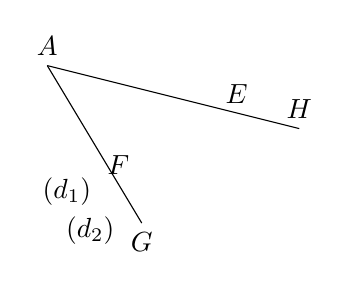
\begin{tikzpicture}[scale = 0.4]
            % \draw[help lines, color=black!30, dashed] (0,0) grid (10,7);        
            \coordinate[label=above:$A$] (A) at (1,6);            
            \coordinate[label=above:$F$] (F) at (3.26,2.24);            
            \coordinate[label=left:$(d_1)$] (d1) at (2.7,2);            
            \coordinate[label=below:$G$] (G) at (4,1);
            \coordinate[label=left:$(d_2)$] (d2) at (3.44,0.76);
            \coordinate[label=above:$E$] (E) at (7.01,4.5);            
            \coordinate[label=above:$H$] (H) at (9,4);
            \tkzDrawLine(E,F);
            \tkzDrawLine(H,G);
            \draw (A)--(H);
            \draw (A)--(G); 
        \end{tikzpicture}
        &
        $\bullet$
        &
        &
        $\bullet$
        &
        $\dfrac{AE}{EH}=\dfrac{EF}{EG}=\dfrac{AF}{GH}$
        \\
        \begin{tikzpicture}[scale = 0.5]
            \begin{scope} [rotate=-10]
            % \draw[help lines, color=black!30, dashed] (0,0) grid (10,7);        
            \coordinate[label=above left:$A$] (A) at (5,6);
            \coordinate[label=below:$H$] (H) at (3.01,1.5);
            \coordinate[label=left:$(d_1)$] (d1) at (2.43,1.26);            
            \coordinate[label=above:$G$] (G) at (5,2);
            \coordinate[label=above:$F$] (F) at (1,5);
            \coordinate[label=left:$(d_2)$] (d2) at (0.4,4.76);            
            \coordinate[label=right:$E$] (E) at (3.67,3);
            \tkzDrawLine(A,H);
            \tkzDrawLine(F,G);
            \tkzDrawLine(F,A);
            \tkzDrawLine(H,G);
            \end{scope}
        \end{tikzpicture}
        &
        $\bullet$
        &
        &
        $\bullet$
        &
        $\dfrac{FE}{FG}=\dfrac{FH}{FA}=\dfrac{EH}{AG}$
        \\        
        \begin{tikzpicture}[scale = 0.5]
            \begin{scope} [rotate=75]
            % \draw[help lines, color=black!30, dashed] (0,0) grid (10,7);        
            \coordinate[label=left:$A$] (A) at (5,6);
            \coordinate[label=right:$H$] (H) at (3.01,1.5);
            \coordinate[label=left:$(d_1)$] (d1) at (2.43,1.26);            
            \coordinate[label=right:$E$] (E) at (5,2);
            \coordinate[label=left:$G$] (G) at (1,5);
            \coordinate[label=left:$(d_2)$] (d2) at (0,4);            
            \coordinate[label=above:$F$] (F) at (3.67,3);
            \tkzDrawLine(A,H);
            \tkzDrawLine(E,G);
            \tkzDrawLine(E,H);
            \tkzDrawLine(A,G);
            \end{scope}
        \end{tikzpicture}
        
        &
        $\bullet$
        &
        &
        $\bullet$
        &
        $\dfrac{AE}{AH}=\dfrac{AF}{AG}=\dfrac{EF}{HG}$
        \\        
    \end{tabular}
    
\end{exercice*}
\begin{corrige}
    %\setcounter{partie}{0} % Pour s'assurer que le compteur de \partie est à zéro dans les corrigés
    \phantom{rrr}
    \begin{multicols}3
        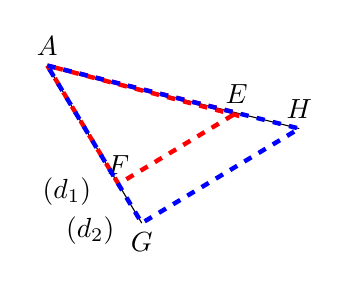
\begin{tikzpicture}[scale = 0.4]
            % \draw[help lines, color=black!30, dashed] (0,0) grid (10,7);        
            \coordinate[label=above:$A$] (A) at (1,6);            
            \coordinate[label=above:$F$] (F) at (3.26,2.24);            
            \coordinate[label=left:$(d_1)$] (d1) at (2.7,2);            
            \coordinate[label=below:$G$] (G) at (4,1);
            \coordinate[label=left:$(d_2)$] (d2) at (3.44,0.76);
            \coordinate[label=above:$E$] (E) at (7.01,4.5);            
            \coordinate (E1) at (7.1,4.4);
            \coordinate[label=above:$H$] (H) at (9,4);
            \tkzDrawLine(E,F);
            \tkzDrawLine(H,G);
            \draw (A)--(H);
            \draw (A)--(G);
            \draw[dashed, color=red, ultra thick](A)--(E)--(F)--(A);
            \draw[dashed, color=red, ultra thick](E1)--(A);
            \draw[dashed, color=blue, ultra thick](A)--(H)--(G)--(A);
        \end{tikzpicture}

        $\dfrac{\textcolor{red}{AE}}{\textcolor{blue}{AH}}=\dfrac{\textcolor{red}{AF}}{\textcolor{blue}{AG}}=\dfrac{\textcolor{red}{EF}}{\textcolor{blue}{HG}}$.
        \columnbreak

        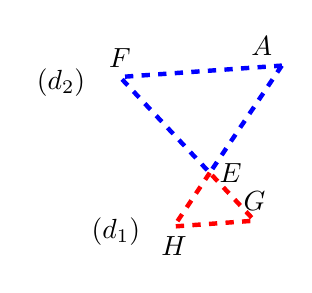
\begin{tikzpicture}[scale = 0.5]
            \begin{scope} [rotate=-10]
            % \draw[help lines, color=black!30, dashed] (0,0) grid (10,7);        
            \coordinate[label=above left:$A$] (A) at (5,6);
            \coordinate[label=below:$H$] (H) at (3.01,1.5);
            \coordinate[label=left:$(d_1)$] (d1) at (2.43,1.26);            
            \coordinate[label=above:$G$] (G) at (5,2);
            \coordinate[label=above:$F$] (F) at (1,5);
            \coordinate[label=left:$(d_2)$] (d2) at (0.4,4.76);            
            \coordinate[label=right:$E$] (E) at (3.67,3);
            \tkzDrawLine(A,H);
            \tkzDrawLine(F,G);
            \tkzDrawLine(F,A);
            \tkzDrawLine(H,G);
            \draw[dashed, color=blue, ultra thick](A)--(E)--(F)--(A);
            \draw[dashed, color=red, ultra thick](E)--(H)--(G)--(E);
            \end{scope}
        \end{tikzpicture}

        $\dfrac{\textcolor{blue}{AE}}{\textcolor{red}{EH}}=\dfrac{\textcolor{blue}{EF}}{\textcolor{red}{EG}}=\dfrac{\textcolor{blue}{AF}}{\textcolor{red}{GH}}$.
        \columnbreak

        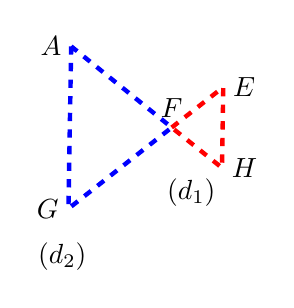
\begin{tikzpicture}[scale = 0.5]
            \begin{scope} [rotate=75]
            % \draw[help lines, color=black!30, dashed] (0,0) grid (10,7);        
            \coordinate[label=left:$A$] (A) at (5,6);
            \coordinate[label=right:$H$] (H) at (3.01,1.5);
            \coordinate[label=left:$(d_1)$] (d1) at (2.43,1.26);            
            \coordinate[label=right:$E$] (E) at (5,2);
            \coordinate[label=left:$G$] (G) at (1,5);
            \coordinate[label=left:$(d_2)$] (d2) at (0,4);            
            \coordinate[label=above:$F$] (F) at (3.67,3);
            \tkzDrawLine(A,H);
            \tkzDrawLine(E,G);
            \tkzDrawLine(E,H);
            \tkzDrawLine(A,G);
            \draw[dashed, color=blue, ultra thick](A)--(G)--(F)--(A);
            \draw[dashed, color=red, ultra thick](F)--(E)--(H)--(F);
            \end{scope}
        \end{tikzpicture}

        $\dfrac{\textcolor{red}{FE}}{\textcolor{blue}{FG}}=\dfrac{\textcolor{red}{FH}}{\textcolor{blue}{FA}}=\dfrac{\textcolor{red}{EH}}{\textcolor{blue}{AG}}$.
    \end{multicols}

    

\end{corrige}

